\documentclass{article}
\usepackage{pgfplots}
\usepackage{listings}
\usepackage{amsfonts}
\usepackage{fancybox, calc}
\lstset{language=Matlab, breaklines=true,
	 basicstyle=\footnotesize}
\lstset{numbers=left, numberstyle=\tiny, stepnumber=1, numbersep=-6pt}
\setlength{\parskip}{\baselineskip}
\renewcommand{\baselinestretch}{1}
\usepackage{amssymb,amsmath}
\usepackage[spanish]{babel}
\usepackage[utf8]{inputenc}
\usepackage[left=4cm,right=3cm,top=4cm,bottom=3cm]{geometry}
\usepackage{graphicx}
\graphicspath{control/}
\setlength{\parskip}{\baselineskip}
\title{INSTITUTO TECNOLÓGICO DE MORELIA\\ **Análisis de un sistema de primer orden**}
\author{Alumnos: Enesto Prado Rodríguez (14120085)\\Juan Pablo Leon Pascual (15122003) \\ \\ Profesor: Gerardo Marx Chávez Campos \\ \\ Materia: Control 1}

\begin{document}
	\maketitle
	\newpage\section{INTRODUCCIÓN}
	Es muy difícil analizar cualitativa mente la transformada de Laplace y la transformada Z, ya que al graficar su magnitud y ángulo a su parte real e imaginaria da como resultado varias gráficas de superficies de dos dimensiones en espacios de tres dimensiones. Por esta razón, es común el examinar la gráfica de la función de transferencia con sus polos y ceros y tratar una vez más una idea cualitativa de lo que hace el sistema.
	Dada a una función de transformación continua, en el dominio de Laplace, H s, o en el dominio discreto de Z, H z, un cero es cualquier valor de s o z para los cuales la función de transferencia es cero, un polo es cualquier valor de s o z para la cual la función de trasferencia es infinita. Lo siguiente da a una definición precisa:
	Ceros
	El valor(es) para z donde el numerador de la función de trasferencia es igual a cero. Las frecuencias complejas que hacen que la ganancia de la función de transferencia del filtro sea cero.
	Polos
	El valor(es) para z donde el denominador de la función de transferencia es igual a cero. Las frecuencias complejas que hacen de la ganancia de la función de transferencia del filtro se infinita.
	
\newpage\section{METODOLOGÍA}

\begin{figure}[h!]
	\centering
	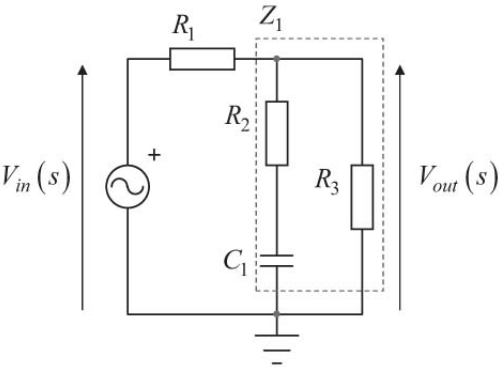
\includegraphics{C:/Users/ERNESTO/Pictures/control/diagracap.png}
	\caption{Diagrama del problema a resolver}
\end{figure}
Capacitor. Analisis por mallas

Malla 1
\begin{equation}
-Vin(t)+R_{1}I_{2}(t)+R_{2}(I_{1}(t)-I_{2}(t))+\frac{1}{c}\int{[I_{1}(t)-I_{2}(t)}]dt=0
\end{equation}
Malla 2
\begin{equation}
\frac{1}{c}\int{[I_{2}(t)-I_{1}(t)}]dt+R_{3}I_{2}(t)+R_{2}[I_{2}(t)-I_{1}(t)]
\end{equation}


Malla 1 

\begin{equation}
-Vin(s)+R_{1}I_{2}(s)+R_{2}(I_{1}(s)-I_{2}(s))+\frac{1}{sc}[I_{1}(s)-I_{2}(s)]=0
\end{equation}


Malla 2
\begin{equation}
\frac{1}{sc}[I_{2}(s)-I_{1}(s)]+R_{3}I_{2}(s)+R_{2}[I_{2}(s)-I_{1}(s)]
\end{equation}

se resuelve el sistema de ecuaciones por igualación

ecuacion 1

\begin{equation}
I_{1}(s)=\frac{Vin(s)+I_{2}(s)[R_{2}+\frac{1}{sc}]}{R_{1}+R_{2}+\frac{1}{sc}}
\end{equation}
ecuacion 2
\begin{equation}
I_{1}(s)=\frac{-I_{2}(s)[\frac{1}{sc}+R_{3}+R_{2}]}{\frac{-1}{sc}-R_{2}}
\end{equation}

igualamos ecuacion 1 y 2

\begin{equation}
\frac{Vin(s)+I_{2}(s)[R_{2}+\frac{1}{sc}]}{R_{1}+R_{2}+\frac{1}{sc}}=\frac{-I_{2}(s)[\frac{1}{sc}+R_{3}+R_{2}]}{\frac{1}{sc}-R_{2}}
\end{equation}


donde
\begin{equation}
I_{2}(s)=\frac{Vin(s)[\frac{-1}{sc}-R_{2}]}{[R_{2}+\frac{1}{sc}][\frac{-1}{sc}-R_{2}]+[\frac{1}{sc}+R_{3}+R_{2}][R_{1}+R_{2}+\frac{1}{sc}]}
\end{equation}

\begin{equation}
Vo(s)=I_{2}(s)R_{3}
\end{equation}

y nos queda

\begin{equation}
\frac{Vo(s)}{Vin(s)}=\frac{R_{3}+R_{2}R_{3}sc}{R_{3}R_{1}sc+R_{3}R_{2}sc+R_{2}R_{1}sc+R_{3}}
\end{equation}

INDUCTOR analisis por mallas
\begin{figure}[h!]
	\centering
	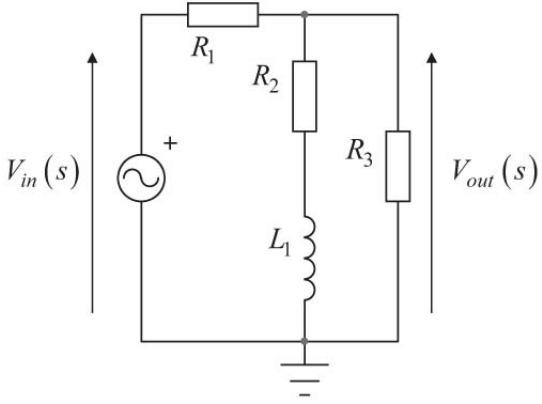
\includegraphics{C:/Users/ERNESTO/Pictures/control/diagraind.png}
	\caption{Diagrama del problema a resolver}
\end{figure}

Malla 1
\begin{equation}
-Vin(t)+R_{1}I_{2}(t)+R_{2}(I_{1}(t)-I_{2}(t))+L\int{[I_{1}(t)-I_{2}(t)}]dt=0
\end{equation}
Malla 2
\begin{equation}
L\int{[I_{2}(t)-I_{1}(t)}]dt+R_{3}I_{2}(t)+R_{2}[I_{2}(t)-I_{1}(t)]
\end{equation}


Malla 1 

\begin{equation}
-Vin(s)+R_{1}I_{2}(s)+R_{2}(I_{1}(s)-I_{2}(s))+Ls[I_{1}(s)-I_{2}(s)]=0
\end{equation}


Malla 2
\begin{equation}
Ls[I_{2}(s)-I_{1}(s)]+R_{3}I_{2}(s)+R_{2}[I_{2}(s)-I_{1}(s)]
\end{equation}

resolvemos por igualacion

ecuacion 1
\begin{equation}
I_{1}(s)=\frac{Vin(s)+I_{2}(s)[R_{2}+Ls]}{R_{1}+R_{2}+Ls}
\end{equation}
ecuacion 2
\begin{equation}
I_{1}(s)=\frac{-I_{2}(s)[Ls+R_{3}+R_{2}]}{Ls-R_{2}}
\end{equation}


igualamos ecuacion 1 y 2

\begin{equation}
\frac{Vin(s)+I_{2}(s)[R_{2}+Ls]}{R_{1}+R_{2}+Ls}=\frac{-I_{2}(s)[Ls+R_{3}+R_{2}]}{Ls-R_{2}}
\end{equation}

entonces queda
\begin{equation}
I_{2}(s)=\frac{Vin(s)[Ls-R_{2}]}{[R_{2}+Ls][-Ls-R_{2}]+[Ls+R_{3}+R_{2}][R_{1}+R_{2}+Ls]}
\end{equation}

y nos queda

\begin{equation}
\frac{Vo(s)}{Vin(s)}=\frac{R_{3}+\frac{R_{2}R_{3}}{Ls}}
{\frac{R_{3}R_{1}}{Ls}+\frac{R_{3}R_{2}}{sc}+\frac{R_{2}R_{1}}{sc}+R_{3}}
\end{equation}

\section{RESULTADOS Y DISCUSIÓN:}
Para la realización o programación de nuestro código tomamos como base el código proporcionado por el profesor en las clases de laboratorio, tal código no lo modificamos tanto, ya que solo era necesario introducirle primero que nada el valor de las variables. 

A continuación veremos los datos que se tomaron en la practica, con el primer circuito que es con el capacitor.
\begin{figure}
	\centering
	\includegraphics{E:/imagenes de control/capacitor.png}
	\caption{código del capacitor}
\end{figure}\\
\begin{figure}
	\centering
	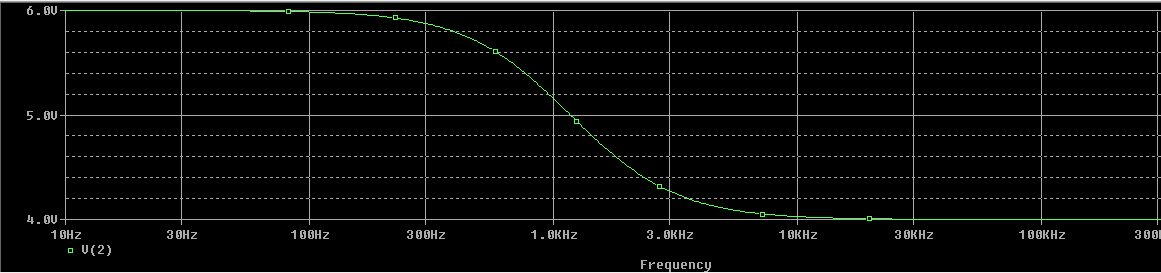
\includegraphics{E:/imagenes de control/grafica del capacitor.png}
	\caption{gráfica del capacitor}
\end{figure}\\
\begin{figure}
	\centering
	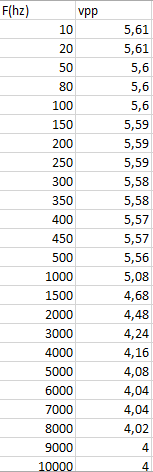
\includegraphics{C:/Users/ERNESTO/Pictures/control/gra2.png}
	\caption{tabla de los datos medidos del capacitor}
\end{figure}\\
Enseguida podemos observar el comportamiento del primer circuito con el capacitor.\\
\begin{figure}
	\centering
	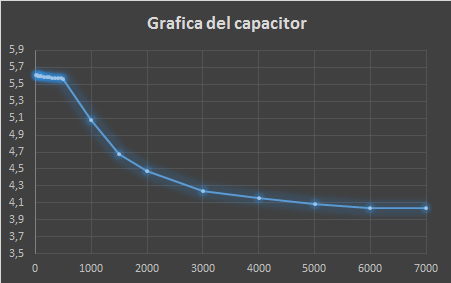
\includegraphics{C:/Users/ERNESTO/Pictures/control/capaci.png}
	\caption{gráfica del capacitor}
\end{figure}\\
Enseguida obtenemos el valor de tao para el capacitor.
\begin{figure}
	\centering
	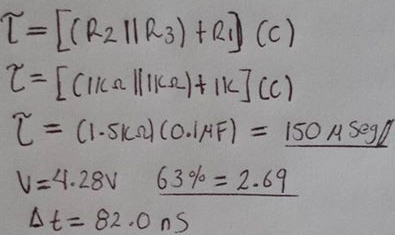
\includegraphics{C:/Users/ERNESTO/Pictures/control/taoca.png}
	\caption{calculo del tao para el capacitor}	
\end{figure}\\
Enseguida podemos observar como se calculo tao con ayuda de los cursores en el osciloscopio.
\begin{figure}
	\centering
	\includegraphics{C:/Users/ERNESTO/Pictures/control/capacitor.jpg}
	\caption{tao al 63}	
\end{figure}\\
A continuación veremos los datos que se tomaron en la practica, con el primer circuito que es con el inductor.

\begin{figure}
	\centering
	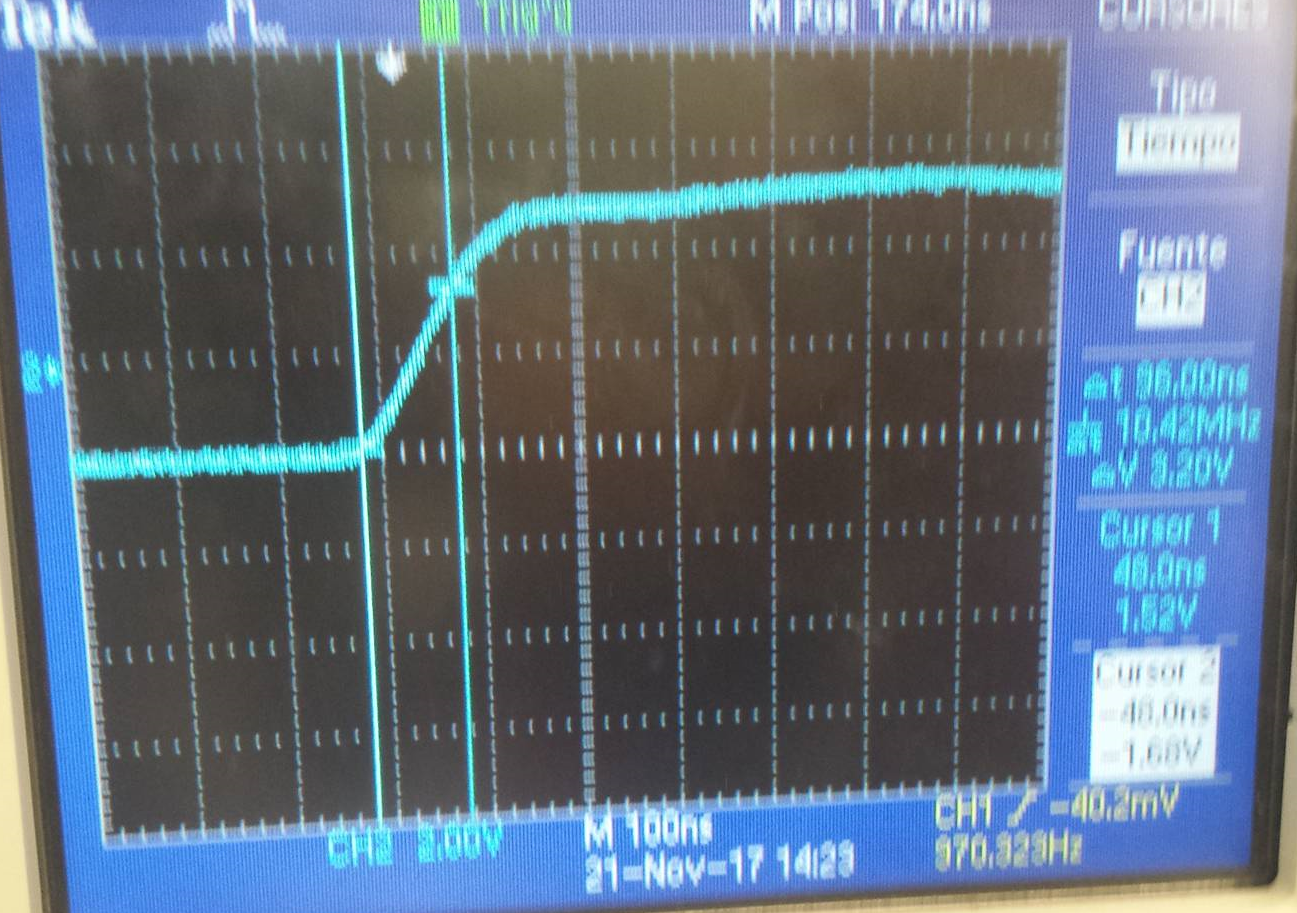
\includegraphics{E:/imagenes de control/inductor.png}
	\caption{código del inductor}
\end{figure}\\
\begin{figure}
	\centering
	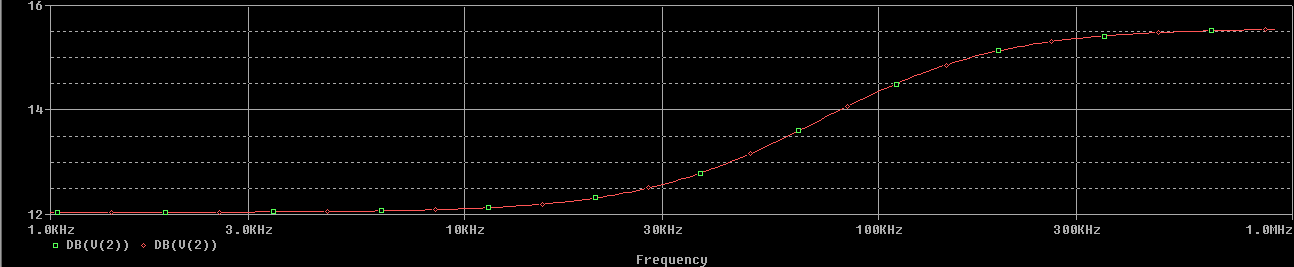
\includegraphics{E:/imagenes de control/grafica del inductor.png}
	\caption{gráfica del inductor}
\end{figure}\\
\begin{figure}
	\centering
	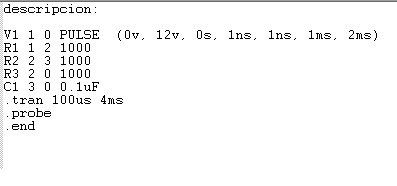
\includegraphics{E:/imagenes de control/pulsante capcitor.png}
	\caption{pulsante capacitor}
\end{figure}\\

\begin{figure}
	\centering
	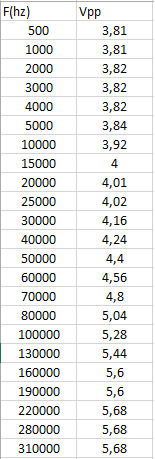
\includegraphics{C:/Users/ERNESTO/Pictures/control/gra1.png}
	\caption{tabla de datos obtenidos del inductor}	
\end{figure}\\
\begin{figure}
	\centering
	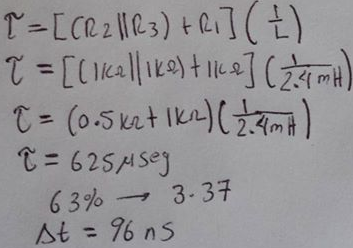
\includegraphics{C:/Users/ERNESTO/Pictures/control/taoind.png}
	\caption{tao del inductor}	
\end{figure}\\
\begin{figure}
	\centering
	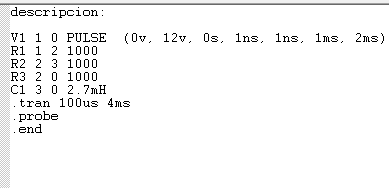
\includegraphics{E:/imagenes de control/pulsante inductor.png}
	\caption{pulsante}	
\end{figure}\\

\newpage
\newpage\section{CONCLUSIÓN}
ERNESTO PRADO RODRÍGUES:

Un requerimiento importante para un sistema de control es que debe ser estable.Esto significa que si al sistema se aplica una entrada de magnitud finita, entonces la salida debería también ser finita y ningún modo infinita, es decir, incrementarse dentro de un límite. Se tratan las condiciones que se deben satisfacer para sistemas estables. Para sistemas lineales el requerimiento de estabilidad se puede definir en términos delos polos de la función de transferencia en lazo cerrado. Los polos son las raíces del polinomio del denominador de la función de transferencia y los ceros las raíces del polinomio del numerador de la función de transferencia.

JUAN PABLO LEÓN PASCUAL

Lo aprendido en clase lo llevamos a la practica donde obtuvimos resultados de tao, implementamos los circuitos anteriores donde se obtuvo  la función de transferencia he hicimos un barrido de frecuencia para obtener la gráfica ya simulada. los resultados obtenido concordaron con las simulaciones de cada circuito.



\end{document}